\documentclass[11pt,twocolumn]{witseiepaper}
\RequirePackage{ifpdf}
\usepackage{amsmath}
\usepackage{amssymb}
\usepackage{KJN}
\usepackage{pdfpages}
\renewcommand*{\bibfont}{\small}

\ifpdf
\pdfinfo{
	/Title (Research Proposal)
	/Author (Alice Yang (597609))
}
\fi

\begin{document}
	\title{Masters Research Proposal - Dimensionality reduction techniques in pattern recognition with different types of x-ray images }
	
	\author{Alice Yang (597609) \thanks{School of Electrical and Information Engineering, University of the Witwatersrand, Private Bag 3, 2050, Johannesburg, South Africa} }
	
	\abstract{The objective of this paper is to propose a two-step system for the detection of bone fractures in order to investigate the performance of the system compared to a single step system. The performance are defined by the speed of its execution, classification accuracy and error rate. The two-step system consists of a dimensionality reduction and a automated decision making process. The objective of the introduction of the dimensionality reduction process is to improve the performance of the automated decision making process during the training and decision making sessions. }
	
	\keywords{Dimensionality Reduction, Neural Networks, Supervised Learning,  Unsupervied Learning, Bone Fractures, Medical Images}
	\maketitle
	\thispagestyle{empty}\pagestyle{empty}
	
	\section{Introduction}
	In medical the field there is an emphasis on the importance of medical diagnosis. In critical cases, an inaccurate diagnosis of a symptom can cost a patient's life. Many diagnosis are performed by trained medical doctors, however they are prone to making mistakes which can be influenced by external factors, such as fatigue and lack of training in the particular field. Automation of medical diagnosis was introduced in the early 1970s \cite{Ramesh2004}. There are many algorithms available in diagnosing patients. The basic algorithm consists of "if... then..." statements. Although the algorithm is simple, the list of conditions in the medical field are endless and as a result the execution time to diagnosis a patient's symptoms is not realistic. There are many pattern recognition algorithms available which are categorized in two categories, namely, unsupervised and supervised. The reasoning behind making use of artificial intelligence is to reduce costs. In this proposal report, section 2 presents the background in the related topics, section 3 describes the problem, section 4 illustrates the proposal methodology, section 5 shows the time management for the proposed research and section 6 concludes the paper. 
	
	An alternative approach in medical diagnosis is to focus on one disease to ensure accuracy and quick response. The use of artificial intelligences can be focussed in one area. The focus of this paper is to detect bone fractures from X-Ray images. There are a selection of tools that can be applied in order to achieve the desired outcome for this investigation. These tools can be in the form of supervised learning, reinforcement, unsupervised learning or a combination of the two. Support Vector Machine and Neural Networks are common tools used in artificial intelligence (AI).
	
	\section{Background}
	The review done by \cite{Mahendran2011} for the automation of bone fracture detection indicated that there are various techniques in pattern recognition that comes in the form of unsupervised, reinforcement and supervised. The challenge found in classification are that there is an information overload and size and dimension are a concern. The problem with information overload is that it becomes to computationally expensive to find crucial information needed for the classification. The size and dimension of the information is a concern because large sizes of data contributes to the number of dimensionality, with high number of dimensions it presents a challenge in the classification process and in turn may require more computational resources.
	
	\subsection{Curse of Dimensionality}
	The main problematic factor affecting the performance in classification is the curse of dimensionality. The curse of dimensionality is a problem due to the sparsity of high dimensional spaces, in which an absurd amount of training data is needed in order to get low variance  estimators \cite{intrator_feature_1992}.
	
	Feature extraction with supervised learning algorithms may seem most desired compared to unsupervised learning algorithms, since supervised learning algorithms have more information about the problem and features. However, unsupervised methods do not suffer the curse of dimensionality as supervised learning does since it makes use of local measures to optimally estimate a single dimensional projection function \cite{intrator_feature_1992}.
	
	\subsection{Dimensionality Reduction}
	The collection of digital data has increased drastically over the past decade, which led to datasets having high dimensionality. The high dimensionality found in datasets affected the performance of data processing algorithms. This is known as the curse of dimensionality \cite{Center2002}. Dimensionality reduction is a process targeted at reducing the dimensionality of the considered dataset by reducing the number of random variables. This process can be divided into two stages, namely Feature Selection and Feature Extraction. Both these stages are crucial for automating bone fracture detection. There are two types of dimensionality techniques, convex and concave techniques. This section focuses on convex techniques. Convex techniques optimizes objective functions that do not contain any local optima, which means that the solution space is convex \cite{Boyd2010}. The objective function is usually in a generalized Rayleigh quotient, which can be expressed in the following form: 
	\begin{equation}
	\phi(\textbf{Y}) = \frac{\textbf{Y}^{T}\textbf{AY}}{\textbf{Y}^{T}\textbf{BY}}
	\label{eq: general objective function}
	\end{equation}
	The function expressed in the form of Equation \ref{eq: general objective function} can be easily optimized by solving a generalized eigenproblem. Convex dimensionality reduction techniques can be subdivided into techniques that perform eigendecomposition on full matrix and sparse matrix. The following section focuses on the eigendecomposition of full matrix. 
	
	\subsubsection{PCA/Classical Scaling}
	Principal Component Analysis (PCA) is a linear technique that performs dimensionality reduction through the process of embedding the data into a linear subspace of low-dimensionality. The low-dimensional representation of the data describes the variance of the data \cite{Jolliffe2016}. During the construction of the low-dimensional representation, PCA does not discard information, instead it creates new characteristics to represent the original characteristics. This is done by searching for characteristics that show as much variation as possible. Additionally, PCA searches for characteristics that allows for the reconstruction of the original characteristics from the new characteristics. According to \cite{van2009dimensionality}, maximizing the variance will result to minimizing the error. Hence, the construction of the low-dimensional representation is obtained by determining mapping  \textbf{M} which maximizes the cost function. The cost function is expressed in Equation \ref{eq: scaling cost function}.
	\begin{equation}
	\phi(\textbf{Y}) = \sum_{ij}(d_{ij}^{2} - ||\textbf{y}_i - \textbf{y}_j||^2)
	\label{eq: scaling cost function}
	\end{equation}
	where 
	
	$||\textbf{y}_i - \textbf{y}_j ||^{2}$ = squared Euclidean distance between low-dimensional datapoints $\textbf{y}_i$ and $\textbf{y}_j$
	
	Eigenvectors and eigenvalues are solved using the eigenproblem expressed in Equation \ref{eq: eigenproblem}. Eigenvectors and eigenvalues are crucial in PCA since eigenvectors assist with determining the correlation between the data points whilst eigenvalues, $\lambda$ dictates the weighted average of the variance for any projection.
	\begin{equation}
	cov(\textbf{X})\textbf{M} = \lambda\textbf{M}
	\label{eq: eigenproblem}
	\end{equation}
	The disadvantage with PCA is that the size of the covariance matrix is dependent on the dimensionality of the original dataset. This means that the size of the covariance matrix is proportional to the number of dimensionalities presented by the dataset, which can result in the inability to compute eigenvectors for very high-dimensional datasets \cite{van2009dimensionality}.
	
	Classical Scaling is an identical technique to PCA, however Classical Scaling searches for the linear mapping \textbf{M} that minimizes the cost function that is expressed in Equation \ref{eq: scaling cost function}. Furthermore, the low-dimensional representation is of the Gram Matrix in which the double-centering pairwise squared Euclidean distance matrix entries are obtained using Equation \ref{gram_enteries}.
	\begin{equation}
	k_{ij} = -\frac{1}{2}(d_{ij}^{2}-\frac{1}{n}\sum_{l}d_{il}^{2} - \frac{1}{n}\sum_{l}d_{jl}^{2} + \frac{1}{n^2}\sum_{lm}d_{lm}^{2})
	\label{gram_enteries}
	\end{equation}
	The disadvantage for both PCA and Classical Scaling is the cost function in Equation \ref{eq: scaling cost function} focuses on retaining large pairwise distances $d_{ij}^2$, whereas retaining the small pairwise distance can be important for minimizing error.
	
	\subsubsection{Isomap}
	Unlike PCA and Classical Scaling where the aim of the techniques is to retain the pairwise Euclidean distances, the Isomap technique attempts to preserves the pairwise
	geodesic distances between datapoints \cite{Zhang2012}. This means that the geodesic distance between $x_i$ and $x_j$ imitates as much of the Euclidean between the low-dimensional representation yi and yj as possible. The low-dimensional representation $y_i$ and $y_j$ are computed using the classical scaling technique, which results in a pairwise geodesic distance matrix. The drawback of the Isomap technique is that it constructs erroneous connections in the neighbourhood graph, G which can affect the performance of the Isomap.
	
	\subsubsection{Kernel PCA}
	Kernel Principal Component Analysis (KPCA) is a technique that makes use kernel functions to map data into high dimensional space, by which the space is manipulated using linear PCA \cite{Cui2012}. KPCA makes use of a mapping function by which it computes the kernel matrix $K$ of datapoints $x_i$ and $x_j$. The entries for the kernel matrix is defined by Equation \ref{eq: kernel matrix enteries}.
	\begin{equation}
		k_{ij} = K(x_i, x_j)
		\label{eq: kernel matrix enteries}
	\end{equation}
	where
	\begin{align*}
		K &= \text{kernel function}\\
		x_i \text{ and } x_j &= \text{input datapoints}
	\end{align*}
	The features defined by the kernel function have a zero-mean. Additionally, the eigenvectors of the covariance matrix $\textbf{a}_i$ which is expressed in Equation \ref{eq: kernel covariance matrix} can be computed, since the eigenvectors of the kernel matrix are related.
	\begin{equation}
		\textbf{a}_i = \frac{1}{\sqrt{\lambda_i}} \textbf{v}_i
		\label{eq: kernel covariance matrix}
	\end{equation}
	The low-dimensional representation is obtained by the projection given by Equation \ref{eq: kernel low-dimensional}.
	\begin{equation}
		\textbf{y}_i = \left\{ \sum_{j = 1}^{n}a_1^{(1)}K(\textbf{X}_j, \textbf{X}_i), ... , \sum_{j = 1}^{n}a_d^{(j)}K(\textbf{X}_j, \textbf{X}_i) \right\}
		\label{eq: kernel low-dimensional}
	\end{equation}
	where
	\begin{align*}
		a_1^{(j)} &= \text{jth value in vector }\textbf{a}_1\\
		K &= \text{kernel function}
	\end{align*}
	A disadvantage with KPCA is that the size of the kernel matrix is proportional square number of instances in the dataset. However despite the obvious disadvantages, KPCA is applied to facial recognition, speech recognition and novelty detection \cite{van2009dimensionality}.
	
	\subsubsection{MVU}
	Maximum Variance Unfolding (MVU) is a technique that aims to preserve as much of the distances and angles between nearby points by studying the kernel matrix. As result it forms a neighbourhood graph, $G$ \cite{Jiang2011}. A quadratic equation is formulated for the "unfolding" transformation. The "unfolding" transformation is where MVU maximizes the sum of the squared Euclidean distances between all the datapoints whilst preserving the distances within neighbouring points. This can be described in Equation \ref{eq: optimization problem}.
	\begin{equation}
		\text{Maximize } \sum_{ij}||\textbf{y}_i - \textbf{y}_j||^{2}
		\label{eq: optimization problem}
	\end{equation}
	\begin{align*}
		\text{Subject to:}
		\begin{cases}
			(1)||\textbf{y}_i - \textbf{y}_j||^{2} = ||\textbf{x}_i - \textbf{x}_j||^{2} , \eta_{ij} = 1 \\
			(2)\sum_{i}\textbf{y}_i = 0
		\end{cases}
	\end{align*}
	MVU reformulates the optimization as semidefinite programming (SDP) over matrix $\textbf{K}$ by defining the inner product of $\textbf{K}_{ij} = \textbf{y}_i \cdot \textbf{y}_j$. Thus the SDP can be written as follows: 
	\newline
	Maximize trace(\textbf{K}) subjected to:
	\begin{equation}
		\begin{cases}
			(1) \textbf{K} \geq 0 \\
			(2) \sum_{ij} \textbf{K}_{ij} = 0 \\
			(3) \textbf{K}_{ii} - 2\textbf{K}_{ij} + \textbf{K}_{jj} = ||\textbf{x}_i - \textbf{x}_j||^{2}, \eta_{ij} = 1
		\end{cases}
	\end{equation} 
	From the first condition $\textbf{K} \geq 0$, it indicates that matrix $\textbf{K}$ is required to be positive semi-definite, since SDP is convex. Thus the low-dimensional representation is obtained by solving the SDP. The main weakness found in MVU is the addition of constraints during optimization, which can result to unsuccessful unfolding of manifold. Although, despite its main weakness it is applied to sensor location and DNA micro-array data analysis \cite{van2009dimensionality}.
	
	\subsubsection{Diffusion Maps}
	Diffusion Maps (DM) is a technique based on defining Markov Random Walk graph \cite{COIFMAN20065}. Markov Random Walk is a description of a random process that consists of the successful random steps applied to a mathematical space. The measurement for the proximity of the datapoints is attained by performing the random walk for a number of iterations. Through the number of iterations, the diffusion distances are obtained in which it is used for the representation of the data in the lower dimension. The purpose of the diffusion distance is to integrate over all the paths presented in the graph. For the construction the diffusion maps graph, the weights of the edges are computed using the Gaussian kernel function. The entries to form matrix \textbf{W} is expressed in Equation \ref{eq: W entries}.
	\begin{equation}
		w_{ij} = e^{-\frac{||\textbf{x}_i - \textbf{x}_j||^2}{2\sigma^2}}
		\label{eq: W entries}
	\end{equation}
	where
	\[\sigma = \text{variance of the Gaussian}\]
	The normalization of matrix \textbf{W} is necessary defining the forward transition probability matrix of dynamical process. The normalized matrix \textbf{W} results in matrix $\textbf{P}^{(1)}$ which is formed using Equation \ref{eq: probability transition}.
	\begin{equation}
		p_{ij}^{(1)} = \frac{w_{ij}}{\sum_{k}w_{ik}}
		\label{eq: probability transition}
	\end{equation}
	By making use of the probability matrix for t iteration $\textbf{P}^{(t)}$, the diffusion distance can be defined in Equation \ref{eq: diffusion distance}.
	\begin{equation}
		D^{(t)}(\textbf{x}_i, \textbf{x}_j) = \sqrt{\sum_{k}\frac{(p_{ik}^{(t)}-p_{jk}^{(t)})^2}{\psi(\textbf{x}_k)^{(0)}}}
		\label{eq: diffusion distance}
	\end{equation}
	where
	\begin{align*}
		\psi(\textbf{x}_i)^{(0)} &= \frac{m_i}{\sum_{j}m_j}
	\end{align*}
	$m_i$ is the degree of the node $\textbf{x}_i$ and can be further defined as follows:
	\[m_i = \sum_{j}p_{ij}\]
	The eigenproblem in which diffusion maps solves is expressed in Equation \ref{eq: diffusion eigenproblem}. 
	\begin{equation}
		\textbf{P}^{(t)}\textbf{v} = \lambda\textbf{v}
		\label{eq: diffusion eigenproblem}
	\end{equation}
	Since the graph is fully connected, the largest eigenvalue is trivial, therefore the corresponding eigenvalue is discarded. The low dimensional representation can be expressed in Equation \ref{eq: low-dimension diffusion}.
	\begin{equation}
		\textbf{Y} = \left\{\lambda_2\textbf{v}_2, \lambda_3\textbf{v}_3,...,\lambda_{d+1}\textbf{v}_{d+1} \right\}
		\label{eq: low-dimension diffusion}
	\end{equation}
	where
	\begin{align*}
		\lambda &= \text{eigenvalues}\\
		\textbf{v} &= \text{eigenvectors}
	\end{align*}
	The applications that diffusion maps have been applied to are shape matching and gene expression analysis.
	
	
	\subsection{Supervised Learning and Neural Networks}
	The goal of supervised learning is to create a mapping function, such that when given new input data a prediction of the output data can be made. The mapping function is generated by with given data sets that consists of inputs with its corresponding outputs. Linear regression, random forest and SVM are popular supervised algorithms.
	
	\subsubsection{Support Vector Machine}
	Support Vector Machine (SVM) is a classifier mainly used for complex classification purposes. In order to separate new data into specified categories, SVM is trained with given labelled data making it supervised learning \cite{Rebentrost2014}. An implementation of SVM classifiers is done in \cite{saha_classifying_2016} where the it is used to classify X-Ray images of the body into five categories, namely, head-neck, body, upper-limb and true-negative. Spatial Pyramid Histogram are used to decipher the medical images which is then used to train the Chi-Kernel based SVM. In general, SVM is used for binary classification \cite{Rebentrost2014}.
	
	\subsection{Neural Network}
	Neural Networks in another common tool selection for AI, whereby it consists of three distinguished layers, the input, hidden and output layer. A general neural network consists of one or two hidden layers. The network is trained before use, which deems it as supervised classification or predictions. In \cite{jyothi_congenital_2016}, the technique implemented is back-propagation neural network (BPNN). The network is trained using a Supervised Delta Learning Rule. The result from the developed technique is a binary outcome in which it indicates whether the subject is normal or abnormal.
	
	For neural network, there are various training method. The most commonly used training method is back-propagation. Another well known training method is feed-forward. The back-propagation training method is used to set weight values associated with the link connection between the input layer and the hidden layer as well as the hidden layer and the output layer. It calculates the gradient of a loss function in terms of all the weights within the neural network. This gradient is used to optimize the method which results in updating the weights within network \cite{Oukrich2016}.
	
	The back-propagation algorithm operates by initially assigning random values to the weights. This is expression is for the datasets modelled as follows. There $n$ input expressed as $X = \left\{X_1, X_2, ... , X_i, ..., X_n\right\}$, the hidden layer nodes are expressed by $H = \left\{H_1, H_2, ... , H_h\right\}$ and a set of $m$ output vector is expressed as $Y = \left\{Y_1, Y_2, ... , Y_j, ... , Y_m\right\}$. Therefore, for each node within the hidden layer, the net input, $net_{k}$ can be expressed in Equation \ref{eq: net input}.
	\begin{equation}
		\label{eq: net input}
		net_{k} = \sum_{i = 0}^{n} w_{ik} X_i
	\end{equation}
	where $w$ is the weight.
	\newline
	The output is computed by applying the logistic function to the net input. Thus the output of each hidden layer node is expressed in Equation \ref{eq: logisitic output}.
	\begin{equation}
		\label{eq: logisitic output}
		Out_{net_k} = \frac{1}{1 + e^{-net_k}}
	\end{equation}
	The outputs of the output nodes can be computed in a similar manner. The objective of the back-propagation algorithm is to minimize the error of the output by adjusting the weight values. To calculate the total error Equation \ref{eq: Error} is used.
	\begin{equation}
		\label{eq: Error}
		e_j(t) = \frac{1}{2} \sum_{j = 1}^{m} (output - target)^2
	\end{equation}
	where $e_j(t)$ is the total error at $j$ for $t$ iteration. 
	\newline
	This means that for every $t$ iteration, the error is calculated and the weights are re-adjusted such that the error is at a minimal. A pre-defined threshold can be used to determine the number of iterations, before the neural network is considered to be trained.
	
	\section{Literature Review}
	The automation of detecting bone fractures is becoming increasingly popular. This is mainly due to the difficulty of applying manual analysis to the increasing volume of image data. The difficulty lies in the lack of human expertise, poor image quality and time. The solution to this problem has been explored by various biomedical and engineering professionals. 
	
	A technique that outlines the fractured bones in an X-ray image of a patient's arm within casting material is present by \cite{Jia_Jiang2006}. The technique divides the image into segments, since the casting material causes a low contrast and high noise ratio within the X-ray image. To eliminate the noise, a geodesic active contour model with global coefficients is applied to the segments of bone region. The global constraint for the model is predefined by the prior shape collected. Feedback for each iteration is provided by a maximum-likelihood function. The experimental results obtained by the authors indicated that the technique produced outlines of the fractured bones on the low contrast X-ray images in a robust and accurate manner.
	
	The authors in \cite{Liang_Pan_Huang_Fan_2010} proposed a technique which makes use of mathematical morphology to identify tibia bone fractures. The technique applies segmentation to the x-ray images by dynamically dividing it into several intervals to determine the smallest intervals with the target. The technique makes use of the Otsu method to automatically threshold the small regions. A statistical method is employed for examining the segments to ensure that accuracy is achieved and to prevent over or under segmentation. The segments of the image are adjusted accordingly to the results obtained from each iteration. The iterations end when the test result conforms to stopping conditions. The segmentation process is then followed by mathematical morphology, in which the target border as well as boundary fractures are extracted. The precise location of fractures is detected by superposing the target border image to extracted skeleton.
	
	An automated fracture detection system in long bones has been developed by the authors of \cite{Donnelley2005}. The system first extracts the edges of the x-ray image using a non-linear anisotropic diffusion method. The diffusion method operates by smoothing the image without discarding crucial information regarding the boundary locations. The second step is to determine parameters for the straight lines that best represent the edges of the long bones. This is done modifying the Hough transform which has an automatic peak detection. To highlight the abnormal regions which includes fractures, the magnitude and direction of the gradient is determined by making use of the calculated parameters.
	
	In \cite{Syiam_Aziem_Soliman2004}, an adaptive interface agent (AdAgen) that incorporates trained agents using neural network is proposed. The neural network is used to build the software interface agent for the detection of fractures in long bones. A semi-intelligent system is provided by the software agent. The results obtained from the simulations indicates that the incorporated agents assists with the performance of the automated fracture detection in leg radiography.
	
	The general approach to classifying the presence of bone fracture involves mapping the data to one of several predefined classes. However, there are challenges presented 
	in the classification technique which are due to information overload and size and dimension of the data \cite{Mahendran2011}. According to \cite{Mahendran2011}, a classification technique is defined as a systematic approach of processing data input by constructing classification models. Examples of classification techniques includes Decision Tree Classifiers, Rule-Based Classifiers, Neural Networks, Support Vector Machines and Na\"{i}ve Bayes Classifiers.
	
	There are various standard classifiers implemented for automating the detection of bone fractures using x-ray images. \cite{Mahendran2012} describes a study done to test the performance of single and combination classifiers. The classifiers used in the study are Back-Propagation Neural Network (BPNN), Support Vector Machine (SVM) and Na\"{i}ve Bayes (NB) classifiers. Contrast, Homogeneity, Energy, Entropy, Mean, Variance, Standard Deviation Correlation, Gabor orientation (GO), Markov Random Field (MRF) and intensity gradient direction (IGD) are features exacted for testing each classifier. The metrics used to evaluate the performance of each classifier are sensitivity, specificity, positive predictive value, negative predictive value, accuracy and execution time. The authors discovered that fusion classifiers enhances the detection capacity. Furthermore, the results indicated that the combination of SVM and BPNN obtained the best performance.
	
	\cite{Mahendran_Enhanced} proposes a four-step system that makes use of fusion-classification techniques to automated the detection of bone fracture specifically for leg bones (Tibia). The four-steps are preprocessing, segmentation, feature extraction and bone detection. The three classifiers during the fusion classification are Feed Forward Back-Propagation Neural Network (BPNN), Support Vector Machine (SVM) and Na\"{i}ve Bayes Classifiers (NB). Through experimentation, the authors stated that the proposed four-step system showed significant improvement in terms of detection rate and speed of classification.
	
	In \cite{ComputerAidedBoneFractureDetection}, the authors proposed a system based on Artificial Neural Network (ANN) for the detection of bone fractures. The system is designed to accept X-ray images as its input. The images are then enhanced using pre-processing techniques. The ANN module is trained using the enhanced x-ray images. "\textit{True Detection Rate}" and "\textit{False Detection Rate}" are used to evaluate the performance of the system. The results that authors obtained for the proposed system indicated that the system had a 89\% success rate.
	
	\cite{lim2004detection} describes an approach for automating the detection of bone fractures in the femur and radius. The system consists of a combinational approach. The first step of the system is to pre-process the input, by extracting features, namely Gabor texture, Markov Random Field texture and intensity gradient. The classifiers implemented for testing are Bayesian classifier and Support Vector Machine (SVM). From experimental results, the combined approach improved the detection rate of bone fractures as well as the classification accuracy compared to a single classification approach.
	
	
	
	There have been studies done which combine the algorithms of supervised and unsupervised. The authors of \cite{neagoe_new_2014} proposed a method which combines both supervised and unsupervised algorithms, name.
	
	The authors of \cite{kottaimalai_eeg_2013} designed a system in which it comprises of Principal Component Analysis(PCA) and Neural Network for the classification of EEG Signals. PCA is a form of unsupervised learning whilst neural network is supervised learning and requires training. The authors compared the correctness of the classification using Neural Network to using Principal Component Analysis with Neural Network. The final outcome from the experimentation is that the correctness of the classification of the Principal Component Analysis with Neural Network is better than Neural Network alone. 
	
	\subsection{Combinational Techniques}
	Studies of improving the common tools in AI have been done by combining the tools. There are two types of combinations, hybrid and non-hybrid multiple classifiers. Hybrid multiple classifiers combines different types of AI algorithms, whereas non-hybrid multiple classifiers only consists of one base algorithm and is replicated multiple times. A hybrid multiple classifier is done by \cite{multiple_classification}, in which the algorithms used are K-Nearest Neighbour, Back Propagation Neural Network (BPNN) and SVM. According to the authors, the each of the AI tools is trained with a different set of data. The decision is based on a voting scheme that is called fusion selection. However, the paper presented in \cite{multiple_classification} performs binary results. In other words, it indicates whether a fracture is present or absent. 
	
	Another AI algorithm to be considered for medical diagnosis is deep learning. According to the author in \cite{LeCun2015}, deep learning has the ability to combat complex problems whereas SVM would not be able to, since SVM works better with small data sets that have few outliers. However, the downfall of deep learning is its learning process, in which it can become tedious and computational demanding. Thus for small data sets, it is more plausible to use an off-shelf classifier such as SVM.
	
	\section{Problem Analysis}
	The modern world has presented the technology to predict human speech as well as digitally categorizing handwritten numbers. However, this technology has not been fully utilized in the medical field. There are many debates surrounding the topic of whether machines are better than doctors. In many cases, the argument for doctors states that those who develop AI do not understand the complexity of medicine and those arguing for the machines say that not many understand how AI operates. However, at the end of the day there are still sick patients waiting to be treated with the right medication or medical care. In order to determine the type of medical care the patient needs a diagnosis must be performed. According to \cite{meyer_physicians_2013}, where studies have been done around the United States, it was reported that doctors correctly diagnosed 55.3\% for easier cases and 5.8\% for more difficult cases. However, this is only one article and more investigation is needed to confirm these numbers. Even so, these numbers still indicate that doctors are not perfect and can mis-diagnosis patients. As a result of mis-diagnosis, the patient is subjected to stress or even life threatening situations should the disease be mis-treated. Therefore there is a large emphasis on accuracy and quick detection of diseases.
	
	There are existing pattern recognition techniques available which have the ability to detect the presence of bone fracture. However, there are large amounts of datasets that is passed into the techniques. These datasets create dimensionality, the more datasets there are the higher the number of dimensionality there are. High number of dimensionalities affects the performance of the techniques. This is known as the curse of dimensionality. 
	
	\section{Proposed Methodology}
	The objective of this research is to propose a system which consists of two steps in order to determine the presence of a fracture within medical x-ray images. The first step is dimensionality reduction and the second step is the automation of the decision making process using neural networks. The dimensionality reduction step is intended to map the data from a high dimensionality to a low dimensionality without loosing any critical information needed for the input into the neural network. The system overview is illustrated in Figure \ref{fig:system overview_2}.
	\newline
	In addition, to developing the two-step system an image pre-processing technique is introduced to the system. This can be seen in Figure \ref{fig:system overview_2}.
	\begin{figure}[!h]
		\centering
		
\includegraphics[scale=0.23]{system_overview_2.png}
		\caption{Block Diagram illustrating an overview of the system with image pre-processing }
		\label{fig:system overview_2}
	\end{figure}
	\newline
	The performance for the system is compared to the performance of a single step neural network. The performances are evaluated by accuracy of detection, error rate, and execution speed. The idea behind comparing the systems is to determine whether there are underlining features in the medical x-ray images that simplifies the training process for the neural network as well as obtaining accurate results in minimal time.
	
	\subsection{Image Pre-Processing}
	The medical image is pre-precessed to de-noise and sharpen the image. The image pre-processing system makes use of both sobel and canny techniques. The system produces a total of 26 images highlighting the defining features in the x-ray image in various ways. The types of images produced are listed in Table \ref{tb: image table} along with the dimensions of each image.
	
	\begin{table}[!h]
		\centering
		\caption{Table showing the types of images produced by image pre-processing system along with the dimensions of each image}
		\label{tb: image table}
		\begin{tabular}{| p{4cm} | c |}
			\hline
			Image (jpg file) & Dimensions (pixels) \\
			\hline \hline
			equalised &  \\
			gamma\_corrected &  \\
			denoised & \\
			sharpened & \\
			hist1 & \\
			hist2 & \\
			bitnot & \\
			bitor & \\
			blur & \\
			a\_contour & \\
			binary\_high & \\
			binary\_inverse & $809 \times 899$ \\
			binary\_low & \\
			canny\_contours\_after\_joining & \\
			canny\_contours\_after\_removing & \\
			i\_cannyx3 & \\
			sobel\_dire & \\
			sobel\_value & \\
			u\_hough & \\
			v\_hough & \\
			w\_hough & \\
			\hline
			binary\_gray & \\
			circle & \\
			circle\_contours & $1200 \times 900$ \\
			gray & \\
			sobel & \\
			\hline
		\end{tabular}
	\end{table}
	Furthermore the image pre-processing system produces csv files for gradients, lines and contours for the i\_cannyx3.jpg image. The dimensions of each extracted feature is shown Table \ref{feature_selection}.
	
	\begin{table}[!h]
		\centering
		\caption{Table showing dimensions of the extracted features from i\_cannyx3.jpg image, where $N_g$ is the total number of values for gradient, $N_l$ is the total number of values for lines and $N_c$ is the total number of values for contours.}
		\label{feature_selection}
		\begin{tabular}{|l|p{2cm}|l|}
			\hline
			Features & Dimensions & Description \\
			\hline \hline
			gradient & $2 \times N_g $ & hough line value, \\
			& & angle (in degrees)\\
			\hline
			lines    & $4 \times N_l $ & $x_{1}$, $y_{1}$ \\
			& & $x_{2}$, $y_{2}$ \\
			\hline
			contours & $2 \times N_c $  & $x$ and $y$ values \\
			\hline
		\end{tabular}
	\end{table}
	
	\subsection{Data Structure}
	The data produced by the image pre-processing system can be structured in two various ways. The first structure consists of making use of all the images produced. This creates a three dimensional (3D) structure for one image. The structure can be represented by $1200 \times 900 \times 26$. A graphical representation of the structure can be seen in Figure \ref{fig: first_structure}.
	\begin{figure}[!h]
		\centering
		
\includegraphics[scale=0.23]{first_structure.png}
		\caption{Data structure using all 26 images produced by the image pre-processing systems}
		\label{fig: first_structure}
	\end{figure}
	
	The second structure is constructed from the three extracted features from the i\_crannyx3.jpg, which are gradient, lines and contours. A simplified graphical representation of the structure is shown in Figure \ref{fig: second_structure}. 
	\begin{figure}[!h]
		\centering
		
\includegraphics[scale=0.23]{second_structure.png}
		\caption{Simplified data structure using the three extracted features from i\_cannyx3.jpg}
		\label{fig: second_structure}
	\end{figure}
	
	\subsection{Dimensionality Reduction}
	For investigation purposes, dimensionality reduction is applied to both data structures to test the performance of the different data structures as well as determining whether there is a defining feature from the x-ray images to determine the presence of a bone fracture.
	
	The first data structure for one image has a 3D structure, $1200 \times 900 \times 26$. Since there are 26 resulting images from one original x-ray image, the dimensionality reduction technique chosen is Principal Component Analysis (PCA) since this is linearly structured whereby only one data element is accessed as a time. 
	
	The first step is to determine the covariance matrix for original x-ray image. The covariance matrix is then used to determine the principal components. The number of principal components is proportional to the number of variables, $n$ within an image. The resultant principal components, $P_n$ are computed by determining the eigenvalues of the covariance matrix. The covariance matrix is in a symmetrical form. The eigenvalues found in the covariance matrix are the variances of the principal components. Since the number of principal component are proportional to the number of variables within an image, this means that there are $n$ eigenvalues. All eigenvalues, $\lambda$ are greater than or equal to zero. The largest eigenvalue corresponds to the first principal component. This applies to the next eigenvalue, until the i-th principal component. Therefore $\lambda_i$ corresponds to the i-th eigenvector.
	
	\subsubsection{Step 1:} The first step is to determine the covariance matrix for each original x-ray image, which has a three dimensional structure. Let the three dimensions be represented by $x$, $y$ and $z$. Thus the covariance matrix, $C$ can be expressed in Equation \ref{eq: covariance matrix}.
	\begin{equation}
		\label{eq: covariance matrix}
		C = 
		\begin{bmatrix}
			cov(x,x) & cov(x,y) & cov(x,z) \\
			cov(y,x) & cov(y,y) & cov(y,z) \\
			cov(z,x) & cov(z,y) & cov(z,z) \\
		\end{bmatrix}
	\end{equation}
	
	The result of $cov(x,x)$, $cov(y,y)$ and $cov(z,z)$ are eigenvalues of matrix $C$ which are the variances of the principal component.
	
	\subsubsection{Step 2:} The eigenvectors $v_1, v_2, v_3, ... , v_i$ corresponding to the eigenvalues $\lambda_1, \lambda_2, \lambda_3, ... , \lambda_i$ are calculated. Assuming that the eigenvalues are in descending order such that: $\lambda_1 \geq \lambda_2 \geq \lambda_3, \geq, ...,\geq \lambda_i$, then $\lambda_1$ is the first principal component and $v_1$ consists of the main characteristics for the given data.
	
	\subsubsection{Step 3:} The principal components that expresses the 26 images can be expressed as follows:
	\begin{equation}
		P_i = \lambda_{i1}Z_1 + \lambda_{i2}Z_2 + ... + \lambda_{in}Z_n
	\end{equation} 
	where $Z_n$ represents the 26 various images of the original x-ray image. 
	
	\subsubsection{Step 4:}
	The low-dimension matrix is constructed by selecting the principal components that consists of the most variations of the data. Therefore the result mapping covariance matrix can be expressed as follows: 
	\begin{equation}
		M = [\lambda v_1, \lambda v_2, ... , \lambda v_n]
	\end{equation} 
	
	\subsubsection{Step 5:} The low-dimension matrix is then constructed as follows:
	\begin{equation}
		Y = M^T \times \text{Original Data}
	\end{equation}
	
	\subsection{Neural Network}
	An artificial neural network consists of three different layers: input layer, hidden layer and output layer. There are weighted connections which link the three layers together. The chosen neural network consists of one hidden layer for simplicity purposes. 
	A graphical layout of the neural network is shown in Figure \ref{fig: neural_network}.
	\begin{figure}[!h]
		\centering
		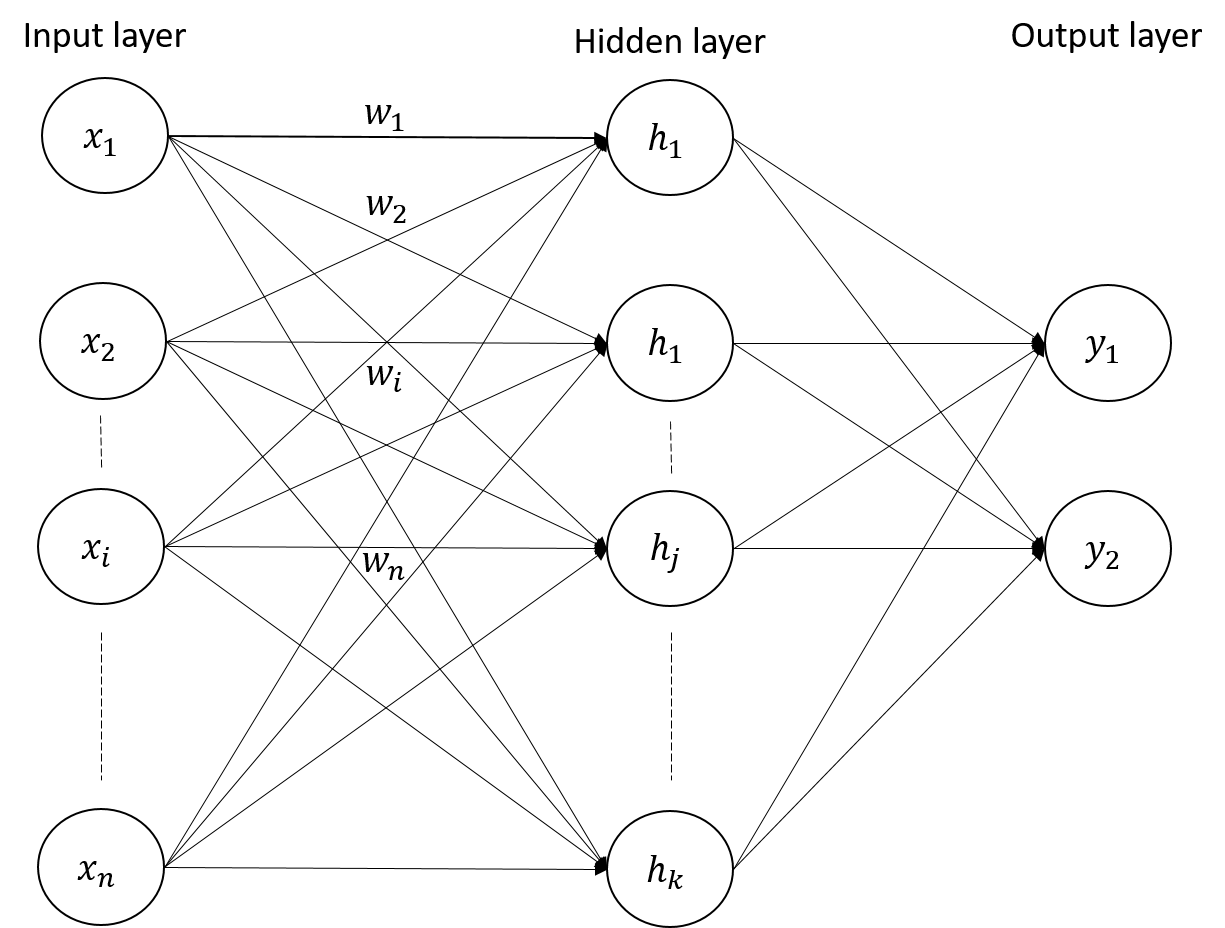
\includegraphics[scale=0.25]{neural_network.png}
		\caption{Neural Network Layout showing the input, hidden and output layers}
		\label{fig: neural_network}
	\end{figure}
	
	The weights are factors which assist with the automated decision making process. The weights values are determined through a training process. The chosen neural network training method is back-propagation. The training process makes use of the resultant matrices from the dimensionality reduction technique. The operations for training the neural network is described below:
	
	\subsubsection{Step 1:} 
	The first step is to initialize the weights in which each weight can be randomly assigned a value (representing the weight), since it will be corrected at a later stage.
	
	\subsubsection{Step 2:}
	The inputs and the desired outputs are defined. The inputs are the matrices obtained from the dimensionality reduction technique, whilst the outputs are the desired outcome result for corresponding input matrices.
	
	\subsubsection{Step 3:}
	The net input into each node, $net_{h_k}$ in the hidden layer is computed as follows for $i = \left\{1, 2, ..., n\right\}$ and $k = \left\{1, 2, ..., k\right\}$:
	\begin{equation}
		net_{h_k} = \sum_{i = 0}^{n} w_{ik}x_i 
	\end{equation}
	
	\subsubsection{Step 4:}
	The output for each node in the hidden layer is calculated by applying the logistic function. The calculation for the first node, $h_1$ is performed as follows:
	\begin{equation}
		Out_{h_k} = \frac{1}{1 + e^{-net_{h_k}}}
	\end{equation}
	
	\subsubsection{Step 5:}
	The net input and output for the nodes at the output layer is computed in the same manner as shown in Step 3 and 4, which given as for $j = \left\{1, 2, ..., k\right\}$ and $m = \left\{1, 2\right\}$:
	\begin{equation}
		net_{y_m} = \sum_{j = 0}^{k} w_{jm}h_j
	\end{equation}
	\begin{equation}
		Out_{y_m} = \frac{1}{1 + e^{-net_{y_m}}}
	\end{equation}
	The output of the nodes, $Out_{y_m}$ are crucial for the next step. 
	
	\subsubsection{Step 6:}
	The objective of back-propagation is to update each weight within the network such that the computed output is as close to the target as possible. This is done by first calculating the total error between the actual output and the target. The total error is computed as follows:
	\begin{equation}
		E_{total} = \sum \frac{1}{2} (target - output)^2
	\end{equation}
	
	\subsubsection{Step 7:}
	The total error is used to adjust the weights within the neural network. This adjustment is performed over $t$ iterations such that the total error is at its minimal. The error minimal value can be a predefined threshold value. The adjustments of the weights are expressed as follows:
	\begin{equation}
		w_{im}(t) = w_{im}(t-1)+\eta\delta_i(t)y_m(t)
	\end{equation}
	where:
	\begin{align*}
		& \delta_i(t) = 
		\begin{cases}
			y_m(t)(1 - y_m(t))\times e_m(t) & m \text{ } \epsilon \text{ output layer}\\
			y_m(t)(1 - y_m(t)) & \text{if not}
		\end{cases} \\
		& 0 < \eta < 1 \\
		& \eta = \text{learning rate} \\
		& e_m(t) = \text{error at node m for t iteration}
	\end{align*}
	
	\subsection{Investigations}
	The performance of the two-step system and the single step system are compared. The performance of both systems are measured by execution speed, accuracy and error rate. The measurement of the execution speed includes the recording of the training speed for the neural network. For the two step system, the data used for training the neural network is the resultant matrices from the dimensionality reduction technique. For the single step system, the original x-ray images are used to train the neural network. 
	
	For further investigation, for the two-step system dimensionality reduction can be performed on the extracted data features: gradient, lines and contours for all 26 images. The resultant matrices from the dimensionality technique can be used to train the neural network. The idea behind using gradients, lines and contours is to avoid analysing the pixels within each image, since the number of pixels is much greater than the number of points given by the three extracted features. The investigation will determine whether using the extracted features are more accurate and less time consuming than using pixels of an image for the detection of a bone fracture.
	
	\section{Time Management and Milestones}
	Table \ref{time_management} and Table \ref{tb: image table} illustrate the tasks that need to completed in order to obtain the results for the research.
	\begin{table}[!h]
		\centering
		\caption{Table showing the time management of the implementation of a bone fracture detection two step system.}
		\label{time_management}
		\begin{tabular}{| c | p{2.5cm} | p{4.5cm} |}
			\hline
			& Period & Task Description \\
			\hline \hline
			1 & Jan 11 - Apr 10 2017 & Work on Research Proposal for submission\\
			\hline
			2 & Apr 11 - Jul 10 2017 & Develop system for image enhancement and feature extraction for x-ray images \\
			\hline
			3 & Jul 11 - Oct 10 2017 &  Develop the system for dimensionality reduction. This includes testing the system\\
			\hline
			4 & Oct 11 - Jan 10 2018 & Develop neural network along with training algorithm for the detection of bone fracture \\
			\hline
			5 & Jan 11 - Apr 10 2018 & Work on first transaction paper \\
			\hline
			6 & Apr 11 - Jul 10 2018 & Integration of both dimensionality reduction model and the neural network model \\
			\hline
			7 & Jul 11 - Oct 10 2018 & Work on second transaction paper\\
			\hline
			8 & Oct 11 - Jan 10 2019 & Work on Dissertation \\
			\hline
		\end{tabular}
	\end{table}
	
	\newpage
	
	\begin{table}[!h]
		\centering
		\caption{Table showing the milestones that need to be achieved in order to complete the research}
		\label{tb: milestones}
		\begin{tabular}{| c | l | p{5cm} |}
			\hline 
			& Date & Task \\
			\hline \hline
			1 & Apr 10 2017 & Submit research proposal for approval\\
			\hline
			2 & Jul 10 2017 & Complete development of image enhancement and feature extraction system \\
			\hline
			3 & Oct 10 2017 & Complete development of the dimensionality reduction model \\
			\hline
			4 & Jan 10 2018 & Complete development of neural network model \\
			\hline
			5 & Apr 10 & Submit first transaction paper \\
			\hline
			6 & Jul 10 2018 & All models fully integrated \\
			\hline
			7 & Aug 10 2018 & All results for research is obtained \\
			\hline
			8 & Oct 10 2018 & Submit second transaction paper \\
			\hline
			9 & Jan 10 2019 & Submit dissertation for approval \\
			\hline
		\end{tabular}
	\end{table}
	
	\section{Conclusion}
	To conclude, the system proposed for the detection of bone fracture consists of two steps. The first step is dimensionality reduction and the second step is the automation based on a neural network model. The objective of implementing a dimensionality reduction process is to improve the performance of the automated bone fracture detection. The performance is measured by both execution speed and training speed, accuracy and error rate. 
	
	\newpage
	\bibliographystyle{witseie}
	\bibliography{standard}
	
\end{document}